This chapter provides an overview and analysis of the related works.
Subsequent sections introduce characteristics of satellite imagery, discuss topics of deep learning and super-resolution.
The following part of the work provides the theoretical background for techniques used in the latter Chapters \ref{ch:scope}, \ref{ch:augmentation}, and \ref{ch:sr-evaluation}.

\section{Characteristics of satellite imagery}
This work centers around super-resolution techniques in the sphere of satellite imagery.
Pictures taken from aerospace devices differ substantially from normal photography.
Multi-image observation is usually favored over single-image (in terms of possible quality of outcome).
Satellites often take a series of photos of a single scene.
This puts emphasis on the multi-image super-resolution techniques in the many-to-one fashion.

Another unique feature of satellite observations is the usual spectral width of the imagery.
Scientific \textit{hyper-spectral} apparatus installed on satellites often acquire photos in a very wide spectrum that may not include frequencies of visible light.
Spectral bands in satellite imagery can contain wavelengths such as infrared, near-infrared, panchromatic\footnote{A spectral range similar to the range of traditional monochromatic grayscale photography.
This range is usually highlighted because of connections with pre-digital imaging of the past century.}, radio frequencies, and more.
This specific kind of image with a large spectral dimension is often called a \textit{hyper-spectral cube} because it can be represented as a three-dimensional tensor (cube) with height, width, and spectral dimensions.
Spectral bands in the cube have the same width and sample adjacent parts of the spectral range.
The \textit{multi-spectral} devices take pictures in multiple different bands of different wavelengths, which often do not border each other.
Multi-spectral images can be treated as discrete sampling points of the spectrum whereas hyper-spectral ones strive to resemble a continuous range of wavelengths \cite{osullivan-2011-spectral}. 
Hyper-spectral images usually feature higher spectral and lesser spatial resolution than multi-spectral pictures \cite{feng-2020-spectral}.
Satellite images with multiple bands are often stored in special file formats or in a series of high bit-depth standard lossless image formats, such as \gls{png} or \gls{tiff}.
These can take up to 13 bands or more in different files per single satellite photography.

One more crucial property of satellite imagery is the \textit{\gls{gsd}} parameter, which denotes a spatial distance between pixels of a digital image.
For example, one-meter \gls{gsd} states that the location of adjacent pixels is one meter apart on the ground.
The \gls{gsd} parameter determines the size of objects visible in the satellite pictures.

Super-resolution for satellite imagery has been developing rapidly in recent years.
The growth of this field was accelerated by the Proba-V super-resolution competition organized by the European Space Agency \cite{esa-proba-competition}.
The challenge lasted from the end of 2018 to June 2019 (over half a year).
The competition consisted in creating a multi-image super-resolution network trained on the Proba-V dataset.
Proba-V is unique in the satellite dataset group---it contains both low-resolution and high-resolution images of the same scenes, making it directly fit for super-resolution network training.
The high-resolution images have \gls{gsd} of $ 1/3 \times 1/3 $ kilometer per pixel and the low-resolution ones feature \gls{gsd} of $ 1 \times 1 $ kilometer per pixel \cite{direckx-2013-proba}.
Architectures submitted in the competition have pushed super-resolution beyond previous baseline performance scores.
A more detailed description of the Proba-V dataset can be found in Section \ref{sec:probav}.

\section{Machine learning for image processing}
\label{sec:machine-learning}
Both the augmentation process and the super-resolution implementations in this work are based on machine learning---especially deep learning.
The following chapters provide an overview of these methods for image processing.

\subsection{Neural networks and deep learning}
\label{sec:neural-nets}
\textit{Machine learning} is a computer science technique that solves problems by fitting models to data using optimization algorithms and statistics.
This approach contrasts with the traditional imperative problem-solving, where algorithms are designed with step-by-step attitude \cite{cholet-2018-deeplearning}.
\textit{Artificial neural networks} are machine learning structures modeled after living organisms and the structure of the brain.
The traditional neural networks consist of layers of densely connected neurons.
Each of the neurons contains a set of inputs with connected weights.
The output of a neuron is the sum of the weighted inputs passed through a nonlinear activation function \cite{bishop-2006-patternrecognition}.
In contrast to more advanced and specialized layers, the classical neurons are often called \textit{dense}, \textit{densely-connected} or \textit{fully-connected}.

Training a neural network in a supervised manner requires a set of examples bounded with ground truth labels.
The fitting process of such a network consists in adjusting the input weights.
Learning is done in steps called \textit{epochs}, during each epoch the training set is passed through the network.
The output of the network is then compared with the ground truth labels.
This is done according to a given \textit{loss function} which serves as a metric between the actual and expected output of the network.
Then the loss is used to optimize the weights via \textit{gradient descent} methods.
The gradients are computed using the \textit{backpropagation} algorithm which is based on the chain rule of derivatives.
There are various loss functions and optimizers to choose from and apply according to the given problem.
In modern deep learning, datasets may be too big to apply backpropagation in one pass.
For this reason, weights are usually updated using small subsets called \textit{minibatches} \cite{goodfellow-2016-deeplearning}.

This kind of machine learning architecture has been initially used with manual feature extraction.
The utilization of a set of predefined filters or feature maps may be an example of this approach in the domain of image processing.
A set of such feature maps would include basic geometric shapes to detect various edge types.
These filters would be matched with regions of the input image.
The results of such an operation are then fed into a neural network or other machine learning algorithm to get the final result of image processing
(an example of this approach can be found in \cite{viola-2001-cascade}).

With the advancements in the machine learning area, a new kind of neural network layer was created---a \textit{convolutional layer} (often abbreviated to \textit{conv layers}).
These layers consist of (one, two, or even three-dimensional) filters that can be convolved with the input image.
However, in  contrast to the manual feature extraction technique, these filters are adjusted in the fitting process of the network \cite{geron-2019-ml} .
Elements in the filter tensor are treated like neuron weights, and they are accommodated during the gradient descent.
This enables the creation of much better performing and flexible image processing neural networks.
Convolutional layers can also be viewed as dense layers with shared weights between groups of pixels.
This way, all pixels can be used in the fitting process without connecting every value in the image with every neuron, which would result in very big and hard-to-train networks \cite{goodfellow-2016-deeplearning}.
A single convolutional layer usually consists of a number of filters.
After passing a standard image through such a layer its depth increases to the number of filters.
It is a common practice to apply a \textit{pooling} (\textit{maximum pooling, average pooling, global pooling}) operation after the convolutional layer to decrease spatial dimension of the image.
Pooling layers reduce the image size by combining multiple pixels into a single one between neural layers (for example, by averaging pixel values).
Alternatively, a convolution with a substantially large stride can be used to shrink the image during a passthrough \cite{springenberg-2015-pooling}.

However, the creation of convolutional neural networks leads to increasing complexity and high numbers of parameters in models.
These complex models demand using very large datasets for the fitting process.
Nowadays, the smallest datasets for training modern neural networks contain thousands of images.
Such trainings require a lot of time and processing power; they usually must be performed using a \gls{gpu} (or even multiple \gls{gpu}s) and may last a few days.
This combination of three factors: complex multi-layered neural networks (often with media-oriented specialized layers), very large datasets (often with many classes and objects), and the utilization of expensive time-consuming trainings constitutes modern \textit{deep learning} \cite{lecun-2015-deeplearning}.
This kind of machine learning has proven, in the last ten years, to hold a revolutionary potential, pushing forward techniques such as image and audio processing beyond what is possible with older methods.
Modern super-resolution, which this work revolves around, is possible thanks to advancements in deep learning.

Generalization capabilities are a valid concern in the field of deep learning.
Machine learning algorithms may be subject to the problem of \textit{overfitting} where the model wights are overadjusted with regard to the training data.
This problem leads to poor performance on data outside of the training set \cite{goodfellow-2016-deeplearning}.
To evaluate the generalization capabilities of a neural network a \textit{test set} is usually utilized.
This dataset contains samples outside of the training data.
One should beware of using test data in any step of the architecture modeling or training process.
The test data should be separate from the model creation, the situation where information from the test set participates in the training process is called \textit{data leakage} \cite{wagh-2018-leakage}.
However, some form of evaluation is desired during the training process.
Often, to prevent overfitting a subset of the training set is separated from the fitting process.
This part of data is called \textit{validation subset} \cite{geron-2019-ml}.
When training loss continues to decrease, but the validation loss increases, the overfitting starts to occur and the training should be stopped.
This work aims to explore the generalization capabilities of super-resolution networks trained on datasets created in different ways.

\subsection{Encoder-decoder mechanism}
\label{sec:encoder-decoder}
Encoder-decoder network architecture is a common pattern in generative image processing.
It is used both in data augmentation networks and super-resolution model utilized in Chapters \ref{ch:augmentation} and \ref{ch:sr-evaluation}.
Encoder-decoder translates the input data into an abstract state during the encoding, then reconstructs it when decoding \cite{sevetlidis-2016-encoderdecoder}.
The mid-point of the architecture usually bottlenecks the information containing compressed-like data.
Convolutional interpretation of the encoder-decoder is commonly used when working with images.
During the encoding process, the depth of input is usually increased and spatial dimensions are shrunken.
This is achieved by subsequent usage of convolutional and pooling layers.
After encoding, the compressed data can undergo some form of processing.
For example, it can be flattened and passed through a fully-connected layer, although this is rarely applied in the super-resolution domain because densely-connected layers break the fully-convolutional \cite{long-2014-fullyconv} nature of a network (meaning that with a dense layer in the middle it cannot process images of varying spatial size).
The decoding process commonly reconstructs depth dimensions into the spatial size by upsampling or transposed convolution.
The output may match the input dimension; however, it is not necessary.
In super-resolution, it is common to output data of a different size than the input.
Encoder-decoder architecture is an appropriate architecture for image-to-image transformations in machine learning.
The inner workings of such an architecture are shown in Figure \ref{fig:encoder-decoder}, where $ x $ and $ y $ denote the input and the output and $ z $ is the encoded hidden state. 
\begin{figure}
    \centering
    \documentclass[tikz]{standalone}
\usepackage[utf8]{inputenc}

\usetikzlibrary{positioning}
\usetikzlibrary{shapes.geometric}

\begin{document}
	
\tikzset{arrow/.style={-stealth}}

\begin{tikzpicture}
	\node[fill=blue!20, minimum width=0.5cm, minimum height=3.5cm] (X) at (0,0) {$\mathbf x$};
	
	\draw([xshift=0.5cm]X.north east) -- ([xshift=2.5cm,yshift=0.5cm]X.east) -- ([xshift=2.5cm,yshift=-0.5cm]X.east) -- ([xshift=0.5cm]X.south east) -- cycle; 
	\node at (1.75,0) {\textsc{Encoder}};
	
	\node[fill=blue!20, minimum width=0.5cm, minimum height=1.0cm] (Z) at (3.5cm,0) {$\mathbf z$};
	
	\draw([xshift=0.5cm]Z.north east) -- ([xshift=2.5cm,yshift=1.25cm]Z.north east) -- ([xshift=2.5cm,yshift=-1.25cm]Z.south east) -- ([xshift=0.5cm]Z.south east) -- cycle;
	\node at (5.25,0) {\textsc{Decoder}};
	
	\node[fill=blue!20, minimum width=0.5cm, minimum height=3.5cm] (Xp) at (7,0) {$\mathbf y$};
	
	\draw[arrow] (X.east) -- ([xshift=0.5cm]X.east);
	\draw[arrow] ([xshift=-0.5cm]Z.west) -- (Z.west);
	\draw[arrow] (Z.east) -- ([xshift=0.5cm]Z.east);
	\draw[arrow] ([xshift=-0.5cm]Xp.west) -- (Xp.west);
\end{tikzpicture}
\end{document}
    \caption{Schematic of encoder-decoder mechanism}
    \label{fig:encoder-decoder}
\end{figure}

The encoder-decoder mechanism is often enhanced with \textit{residual connections}.
These are often called \textit{skip connections} because they form parallel branches in networks that skip certain operations \cite{cholet-2018-deeplearning}.
These skip routes are then summed with the result of an operation, resulting in the additional direct flow of information during the forward pass and a direct gradient flow on the backward pass.
Residual connections applied between arms of an encoder-decoder create what is called a \textit{U-Net} architecture \cite{ronnenberger-2015-unet}.
In the case of super-resolution processing, the forward skips can be viewed as routes for transporting unprocessed low-frequency information.
This information can be used during the decoding step in the encoder-decoder scheme.

\subsection{Generative Adversarial Networks}
\label{sec:gans-overview}
In recent years, a new approach to training generative neural networks has emerged.
The traditional supervised learning described in the previous sections consists in providing the network with an input sample and comparing the generated output with a ground truth label to compute the loss value.
The \textit{\gls{gan}} approach requires creating two networks, a \textit{generator}, and a \textit{discriminator} \cite{goodfellow-2014-gans}.
The former is tasked with generating data, while the latter learns to differentiate images created by the generator from real ones.
In the \gls{gan} scheme, the discriminator learns like a traditional binary classifier---it is provided with real and generated images, which are labeled accordingly.
Then the discriminator loss is computed using standard classification metrics like \textit{binary cross-entropy}.
However, the generator learns in a more unique way; it creates an output image that is fed into the discriminator.
The generator loss is calculated depending on how well it produces data that may be classified as \textit{real} by the discriminator.
If the generated image is recognized as a \textit{fake} one, the generator receives a big penalty in the form of a large loss.
The inner-workings of a \gls{gan} network can be visualized in the form of a graph, as in Figure \ref{fig:gan-training}.
\begin{figure}
    \centering
    \documentclass[tikz]{standalone}
\usepackage[utf8]{inputenc}

\usetikzlibrary{positioning}
\usetikzlibrary{shapes}
\usetikzlibrary{calc}

\begin{document}
	
\tikzset{arrow/.style={-stealth}}

\begin{tikzpicture}[ampersand replacement=\&]
   	\node[text width=0.25cm] at (-2.5,0) (X) {$ \mathbf x $};		 
    \node[rectangle, rounded corners, draw, fill=blue!20, minimum height=1cm] at (0,0) (G) {\textsc{Generator}};	
    \node[rectangle, rounded corners, draw, minimum height=1cm] at (3,0) (S1) {\textsc{Sample}};
    
    \node[text width=0.5cm] at (0.75,3) (Y) {$ \mathbf y_{gt} $};		 
    \node[rectangle, rounded corners, draw, minimum height=1cm] at (3,3) (S2) {\textsc{Sample}};
    
    \node[rectangle, rounded corners, draw, fill=blue!20, minimum height=1cm] at (6,1.5) (D) {\textsc{Discriminator}};
    
    \node[text width=2cm] at (10,1.5) (O) {\textsc{Real/Fake Prediction}};
     
    \path[arrow] (X) edge (G)
    (G) edge (S1)
    (S1) edge (D.south west)
    (Y) edge (S2)
    (S2) edge (D.north west)  
    (D) edge (O)
    ;
\end{tikzpicture}

\end{document}
    \caption{Schematic of a \gls{gan} network inner-workings}
    \label{fig:gan-training}
\end{figure}

\gls{gan}s can have many variations, the most common type utilizes unsupervised or semi-supervised data generation.
This means that in many \gls{gan}s the generator can be fed with values from proper random distribution (often called \textit{latent space}) to generate new data.
The ability to create images without direct input is a great advantage of adversarial networks.

In general, adversarial network architectures provide vast generative capabilities.
For this reason, \gls{gan}s are widely used for data augmentation and creation \cite{bulat-2018-supergan, sundaram-2021-gangen, shorten-2019-augmentation, perez-2017-augmentation}.
A variant of \gls{gan} architecture is later used in this work for creating super-resolution training data in Chapter \ref{ch:augmentation}.

\subsection{Measuring quality of image-generating neural networks}

Both super-resolution networks and data augmentation networks input and output images.
Quantitative evaluation of such networks requires comparing two images---the network output and the ground truth reference image.
Images are usually compared using metrics like \textit{\gls{mae}}, \textit{\gls{mse}}, and \textit{\gls{psnr}}.
These calculate the error between pairs of corresponding pixels in different ways.
However, these metrics may be insufficient for super-resolution-related problems.
Calculating pixel-wise differences does not resemble the way humans estimate image quality.
Images of varying perceived quality can have the same \gls{psnr}s compared to the reference image.

To measure image similarity in a more reliable way \textit{\gls{ssim}} \cite{wang-2004-ssim} was introduced.
\gls{ssim} calculates image quality in three main components:
\begin{itemize}
	\item Average \textit{luminance}.
	\item \textit{Contrast} as the standard deviation of pixels.
	\item \textit{Structure} as the luminance difference divided by the standard deviation.
\end{itemize}
However, these values are not calculated globally.
Instead, \gls{ssim} values are measured using windows with pixel weights determined by Gaussian distribution.
Values of \gls{ssim} components are combined using a compound formula.
The precise mathematical description of the \gls{ssim} metric can be found in \cite{wang-2004-ssim}.
Advantages of \gls{ssim} render it suitable for super-resolution-related image quality evaluation.

However, modified versions of the previously mentioned traditional metrics can also be useful for image comparison, one of them being the \textit{cPSNR} score.
The traditional \gls{psnr} has the potential drawback of being sensitive to the bias in image brightness.
This metric equalizes the average brightness of compared images before calculating standard \gls{psnr} to alleviate this problem.
The improved version of \gls{psnr} was introduced and used for scoring in the Proba-V super-resolution competition \cite{esa-proba-competition}.
Various of the mentioned metrics are used in this work, in accord with specific requirements of each step in the augmentation and super-resolution training process.

\subsection{Image registration}
\label{sec:registration}
Another challenge often encountered during super-resolution training and evaluation consists in aligning image pairs correctly.
Often two images that are to be compared are slightly shifted; it is common for these dislocations to lie in the subpixel domain.
The process of aligning two similar images is called \textit{image registration}.
Registration can be performed either with traditional or deep learning-based algorithms.
To register the subpixel translations, images can be upscaled before using a matching algorithm.

Registration algorithms can be divided by the applied methodology of image processing.
The first group of methods works on image features and properties.
These algorithms can detect image area characteristics like boundary regions, corners and frequency properties.
Image features can also be detected by similarity measures and image descriptors like \textit{\gls{sift}}, \textit{\gls{surf}}, and statistical properties, e.g., \textit{cross-correlation} (more detailed description of various methods can be found in \cite{jain-2015-registration}).
Pictures can also be characterized by frequency-domain-based traits like \textit{phase-correlation} \cite{guizar-2008-registration}.
This method utilizes a two-dimensional \textit{Fourier transform} on images and is later used in this work (Chapter \ref{ch:augmentation}).

Another branch of image registration techniques takes advantage of modern machine-learning technologies.
These can utilize approaches like deep learning with similarity metrics or unsupervised trainings \cite{haskins-2020-deepregistration}.
A modified version of an image inpainting deep neural network can be used as a well-working registration algorithm \cite{deudon-2020-highresnet, zhaoyi-2018-shiftnet}.
A more detailed explanation of such an approach is included in Section \ref{sec:shiftnet}.

\subsection{Data augmentation in machine-learning}
\label{sec:data-augmentation-in-ml}
Data augmentation techniques are briefly characterized in the introductory part (Section \ref{sec:augmentation-introduction}).
However, this field is a very wide area of research, ranging from applying simple modifications to existing samples to generating synthetic datasets \cite{kar-2019-synthetic}.
Traditional augmentation techniques include operations like zooming, resizing, shifting, flipping, rotating, distorting, adding noise, random erasing, image mixing, applying predefined filters, modifying colors, and exposure.
Data augmentation is useful for preventing overfitting and training complex networks on relatively small datasets \cite{shorten-2019-augmentation}.
These operations may be application-specific.
To give an example, one should beware of distorting or flipping data containing constrained geometry, like road signs.
The artificial data should resemble real-life data as much as possible. 

The traditional augmentation techniques lead to great results; however, more modern approach based on deep learning can be used to widen data generation capabilities.
The popularization of \gls{gan} networks has led to great advancements in data generation.
Thanks to the adversarial networks entirely artificial samples can be generated \cite{sundaram-2021-gangen} even online during the training process \cite{bulat-2018-supergan}.

\section{Overview of super-resolution techniques}
As mentioned in Chapter \ref{ch:introduction} super-resolution techniques can be divided into single and multi-image categories where one or many low-resolution images are turned into a high-resolution one.
The latter is a more advanced technique, which utilizes multiple low-resolution
images of the same scene to produce one high-resolution picture.
The usual approach is to utilize multiple low-resolution images that are slightly shifted (in the subpixel domain).
Data from these multiple images is merged together to produce an image of greater quality \cite{kawulok-2019-multisr}.
This approach can lead to the best results in super-resolution.
In some scenarios, the data fusion can lead to the recreation of high-resolution details that are hardly visible in any single low-resolution image.
In the case of multi-image super-resolution, better image quality comes at a cost of obtaining a series of input pictures instead of one, as it is in the single-image approach.

The simplest super-resolution methods predate deep-learning techniques and utilize interpolation for multi-image data.
Multiple low-resolution images with subdomain shifts can be used to achieve more detailed interpolation for missing values in the reconstructed high-resolution picture \cite{park-2003-sr}.
Nowadays super-resolution is mainly done with deep learning techniques which undergo rapid development.
Deep learning-based super-resolution can be divided in regard to: supervision (supervised or unsupervised learning), application domain, network architecture, learning strategy, and evaluation technique \cite{wang-2019-srsurvey, bashir-2021-srreview}.
Machine learning techniques that enable modern super-resolution are discussed in Section \ref{sec:machine-learning}.
There are many deep learning-based modern super-resolution models that may vary in architecture.
Examples of such networks are: \textit{\gls{rams}} \cite{salvetti-2020-rams}, \textit{HighRes-net} \cite{deudon-2020-highresnet}, and \textit{\gls{deepsum}} \cite{moloni-2020-deepsum}.
An in-depth analysis of a super-resolution neural network is provided in Section \ref{sec:sr-highresnet}.

\subsection{Super-resolution with HighRes-net}
\label{sec:sr-highresnet}
In recent years many super-resolution architectures have emerged due to advancements in deep learning techniques.
At the moment, \gls{rams} architecture achieves one of the best scores.
However, in this work HighRes-net architecture is utilized.
HighRes-net, which is a few months older, achieves slightly worse results; however, it is simpler and faster to train \cite{paperswithcode-ranking}.
Because the aim of the work is to compare different data generation techniques, not the super-resolution algorithms themselves, the more manageable architecture was chosen.
A brief description of the more sophisticated architecture is also given to provide a wider context.

\subsubsection{Architecture overview}
HighRes-net \cite{deudon-2020-highresnet} is a super-resolution network based on generative deep learning.
It falls into the category of \textit{\gls{mfsr}} algorithms, which takes a \textit{many-to-one} (or \textit{multi-image}) approach to output generation.
In \gls{mfsr} systems input is a series of images, taken with a slight shift, and in different moments in time.
The input series contains more information, than a single image, as a result of random displacements, noise disturbances, and atmospheric conditions.
\gls{mfsr} tackles the problem of aliasing in sampled data.
Low-frequency parts of the image, with large geometry and little detail, do not differ much between many images.
However, \gls{mfsr} is crucial when enhancing small details.
Upscaling small geometry from a single image can be non-reliable due to aliasing.
Applying \gls{mfsr} techniques and multiple low-resolution images fusion leads to de-aliasing information contained in the images.
HighRes-net processing is divided into four subtasks:
\begin{enumerate}
	\item \textbf{Co-registration}, which estimates relative geometric differences between input images. These include divergences, due to shifts, rotations, deformations, etc.).
	\item \textbf{Fusion}, which combines multiple input images into a single one that is more refined.
	\item \textbf{Up-sampling}, which upscales an input low-resolution image into a high-resolution one.
	\item \textbf{Registration-at-the-loss}, which estimates relative geometric differences of high-resolution prediction and ground truth, for more representative loss calculation. After calculating the shift between the super-resolution output and the reference image, they are aligned using Lanczos resampling, and then the loss is measured.
	    The registration and alignment are learned by a model inspired by the \textit{ShiftNet} network architecture.
\end{enumerate}
The unique feature of HighRes-net is that all of its parts are learned in a single fit in an end-to-end fashion.

\subsubsection{Super-resolution inference process}
The inference pipeline of HighRes-net is shown in Figure \ref{fig:highresnet-inference}.
The consecutive paragraphs will walk through each step in the process and explain how super-resolution is performed.
\begin{figure}
    \centering
    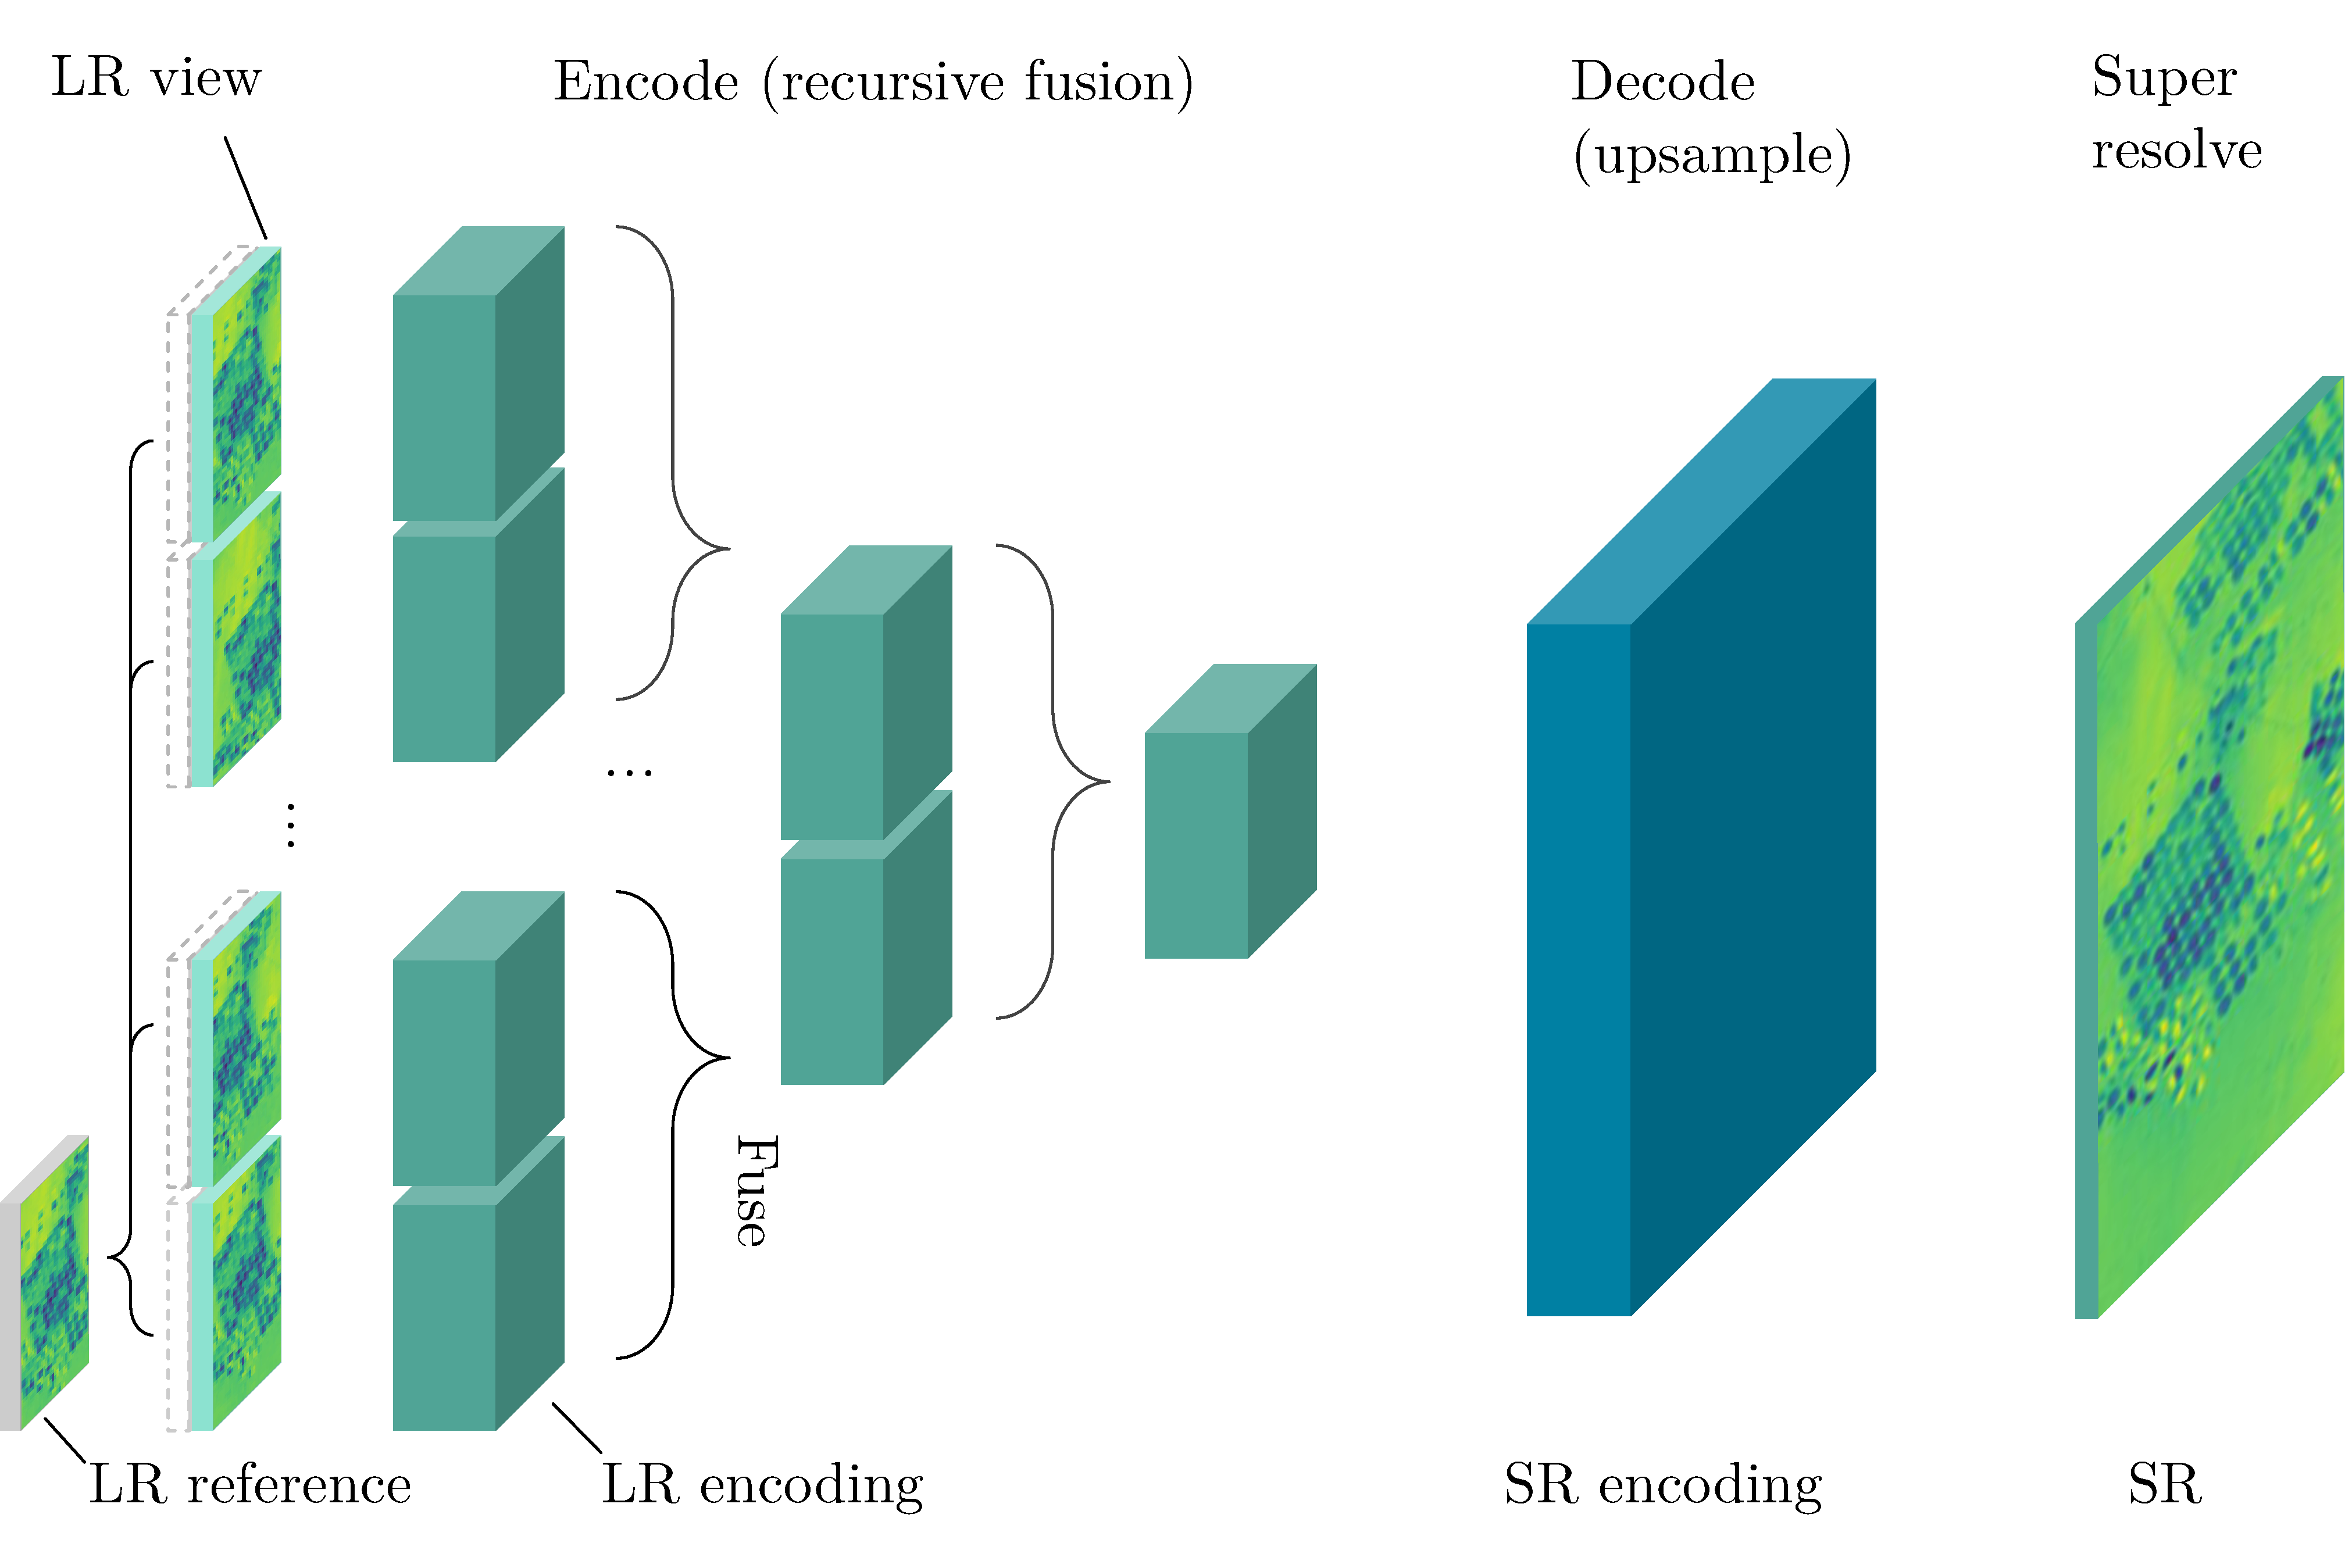
\includegraphics[width=0.9\textwidth]{high_res_net_inference}
    \caption{Schematic of inference in HighRes-net \cite{deudon-2020-highresnet}}
    \label{fig:highresnet-inference}
\end{figure}

The key element of HighRes-net is achieving \textit{multi-frame super-resolution} by \textit{recursive fusion}.
Image generation is done by a neural network organized in an encoder-decoder scheme.
The input of the encoder is constructed from a series of low-resolution images.
If necessary, the input set is padded with zero-valued images to ensure that the number of low-resolution images is a power of 2, which is required by the network architecture.
For each input series, a \textit{reference image} is computed using median values of images.
Then the reference picture is paired with the input images.
Each low-resolution and reference pair is processed through an embedding function.
Embedding layers consist of a convolutional layer and two residual blocks with \textit{\gls{prelu}} activations.
For input of length \textit{n}, the output of the encoding consists of \textit{n} images, each convolved with the reference image.
In this scheme, embedding learns to perform a process called \textit{implicit co-registration}, which is responsible for adjusting geometric differences between images in the input.
It is important to notice that the embedding block is a single instance shared between input pairs.

The next step in the HighRes-net architecture is \textit{recursive-fusion}.
In this process output images are recursively fused together, pair by pair.
The fusion operation consists of two steps---co-registration of the input pair and the actual fusion.
The co-registration of fused images is similar to the co-registration of the input-reference pairs.
It is done by a convolutional layer with \gls{prelu} activation and two residual layers.
Then the fusion itself is done, again by a combination of a convolutional layer and \gls{prelu} (this part does not include local residual layer).
The whole co-registration-fusion includes a residual connection.
As in the embedding block, the fusion operator has a single instance that is shared for all steps of the recursion.

The last step of super-resolution process is to upscale the image by decoding the hidden state.
This is done with a transposed convolutional layer with \gls{prelu} activation.
The transposition of the output of convolution makes the data grow in spatial dimensions, instead of the usual increase of depth when convolving.
The final image is constructed by applying convolution of size one.

\subsubsection{Registered loss calculation}
\label{sec:shiftnet}
As stated before, registration is an important part of HighRes-net architecture.
It is especially crucial at the loss calculation step.
Without registration, the network would learn to output blurry images as a result of a shift between predictions and targets.
Previous steps of HighRes-net include an \textit{implicit co-registration}, where registration mechanisms learned by the network do not have to be necessarily based on shifts, but also other geometric distortions.
During the evaluation it is desired to register image shifts explicitly, thus the \textit{registration-at-loss} differs from the registration performed during encoding and fusion.
At the final step, the subpixel registration is done by the \textit{ShiftNet-Lanczos} network.
ShiftNet \cite{zhaoyi-2018-shiftnet} was introduced before HighRes-net, in a separate research.
It was created for image inpainting\footnote{\textit{Inpainting} is a process of reconstructing or readjusting missing or damaged parts of an image.} via \textit{Deep Feature Rearrangement} technique.
Because this kind of filling-in missing picture areas works by reusing and transferring existing data, it is suitable to be used as a registration mechanism.
It implements a modified \textit{U-Net} \cite{ronnenberger-2015-unet} architecture.
As mentioned in Section \ref{sec:encoder-decoder}, U-Nets follow the encoder-decoder pattern with multiple residual connections.
Pairs of convolution and deconvolution layers in the contracting and expanding arms of a U-Net feature a residual connection.
The ShiftNet variant of U-Net architecture contains an additional \textit{shift} operation for one of these residual connections.
More about ShiftNet can be found in the publication that introduces it.

\subsection{Other super-resolution architectures}
As mentioned, other super-resolution architectures are available, with \gls{rams} \cite{salvetti-2020-rams} being one the best performing.
\gls{rams} utilizes a novel technique called \textit{feature attention mechanism}, which enables the network to focus on high-frequency information that can be used to produce more detailed outputs.
This leads to overcoming main locality limitations of convolutional operations.
Mechanisms used in \gls{rams} are specifically aimed at multi-image super-resolution of remote sensing data.
\gls{rams} approach takes into account the nature of satellite imagery---relatively low spatial resolution and high depth and temporal resolution.
The attention mechanism works with three-dimensional convolutions to explore all possible directions.
This architecture puts emphasis on simultaneous data exploration from spatial and temporal dimensions resulting in the best quality of multi-image super-resolution.

\section{Resizing images with interpolation techniques}
Image resizing is a relevant topic in super-resolution, as a reference point and a tool for visualization.
It is useful as a visual baseline for super-resolution.
Traditional image resizing algorithms use interpolation to enable changing image dimensions; however, they do not create new details in the image.
A well-working super-resolution should recreate missing features when enhancing images.
Thus, it is expected that any super-resolution algorithm gives better results than image interpolation techniques.
In this work, image interpolation is used for comparisons during both the augmentation and super-resolution processes.

\subsubsection{Bicubic interpolation}
\textit{Bicubic interpolation} is one of the most prominent image interpolation techniques.
Compared to other interpolation methods it is regarded as the most advanced and time-consuming of the commonly used solutions \cite{han-2013-interpolation, teoh-2008-inrepolation}.
This interpolation mode fills missing values by fitting third-degree polynomials between existing pixels.
The gradients of existing values are taken into account during the fitting process, so the interpolation splines' steepness matches the existing derivatives.
Bicubic interpolation is usually calculated in neighborhoods of four by four pixels.
Fitting polynomials to existing pixels may lead to \textit{overshooting} values.
This phenomenon often causes a slight increase in local contrast, which overall increases the \textit{acutance} (perceived sharpness) of an image.
Other image resizing modes operate on a simpler basis or consist in fitting simpler interpolation functions.
For this reason, bicubic is the most advanced and often best out of the common solutions.

\subsection{Other interpolation techniques}
The bicubic interpolation has been chosen as the main reference point; however, there are other popular image resizing techniques that may be taken into account in comparisons.

The \textit{nearest neighbor interpolation} is the simplest out of widely used techniques.
In this approach, the missing points are filled in with values of the closest existing pixels.
This technique often resolves in jagged edges and coarse details.

Another widely used approach is \textit{bilinear interpolation}.
The bilinear mode works similarly to bicubic one; however, it operates on simpler terms.
Instead of fitting polynomials, it uses straightforward linear functions to find missing values.
For his reason, it cannot take into account image gradients and often results in a less plausible outcome.
Furthermore, in contrast to the bicubic interpolation, bilinear usually operates in two by two neighborhoods.

\textit{Lanczos} is another interpolation method, with greater complexity and quality similar to bicubic.
In contrast to other techniques, it uses sinus function for interpolation.
Fitting is done using \textit{Lanczos filters} which may vary in function order and neighborhood size.

\section{Image visualisation techniques}
The following chapters will include many visualizations and image previews.
They often include a side-by-side comparison between high and low-resolution images of the same scene that were generated using different methods.
When computers display single-channel images (like the pictures presented in this work), a colormap is often used.
The most popular colormap is grayscale which displays white for maximal values, black for minimal values, and shades of gray in between.
To improve the visibility of details, a yellow and blue colormap called \textit{Viridis} \cite{rudis-viridis} is mainly used in this work.
Viridis is an example of a \textit{Perceptually Uniform Color Map} \cite{kovesi-2015-colormaps}, which aims to guarantee an even perceived contrast of all color shades in the map.
An example of Proba-V satellite image with Viridis colormap applied is shown in Figure \ref{fig:viridis}.
\begin{figure}[htb]
	\centering
    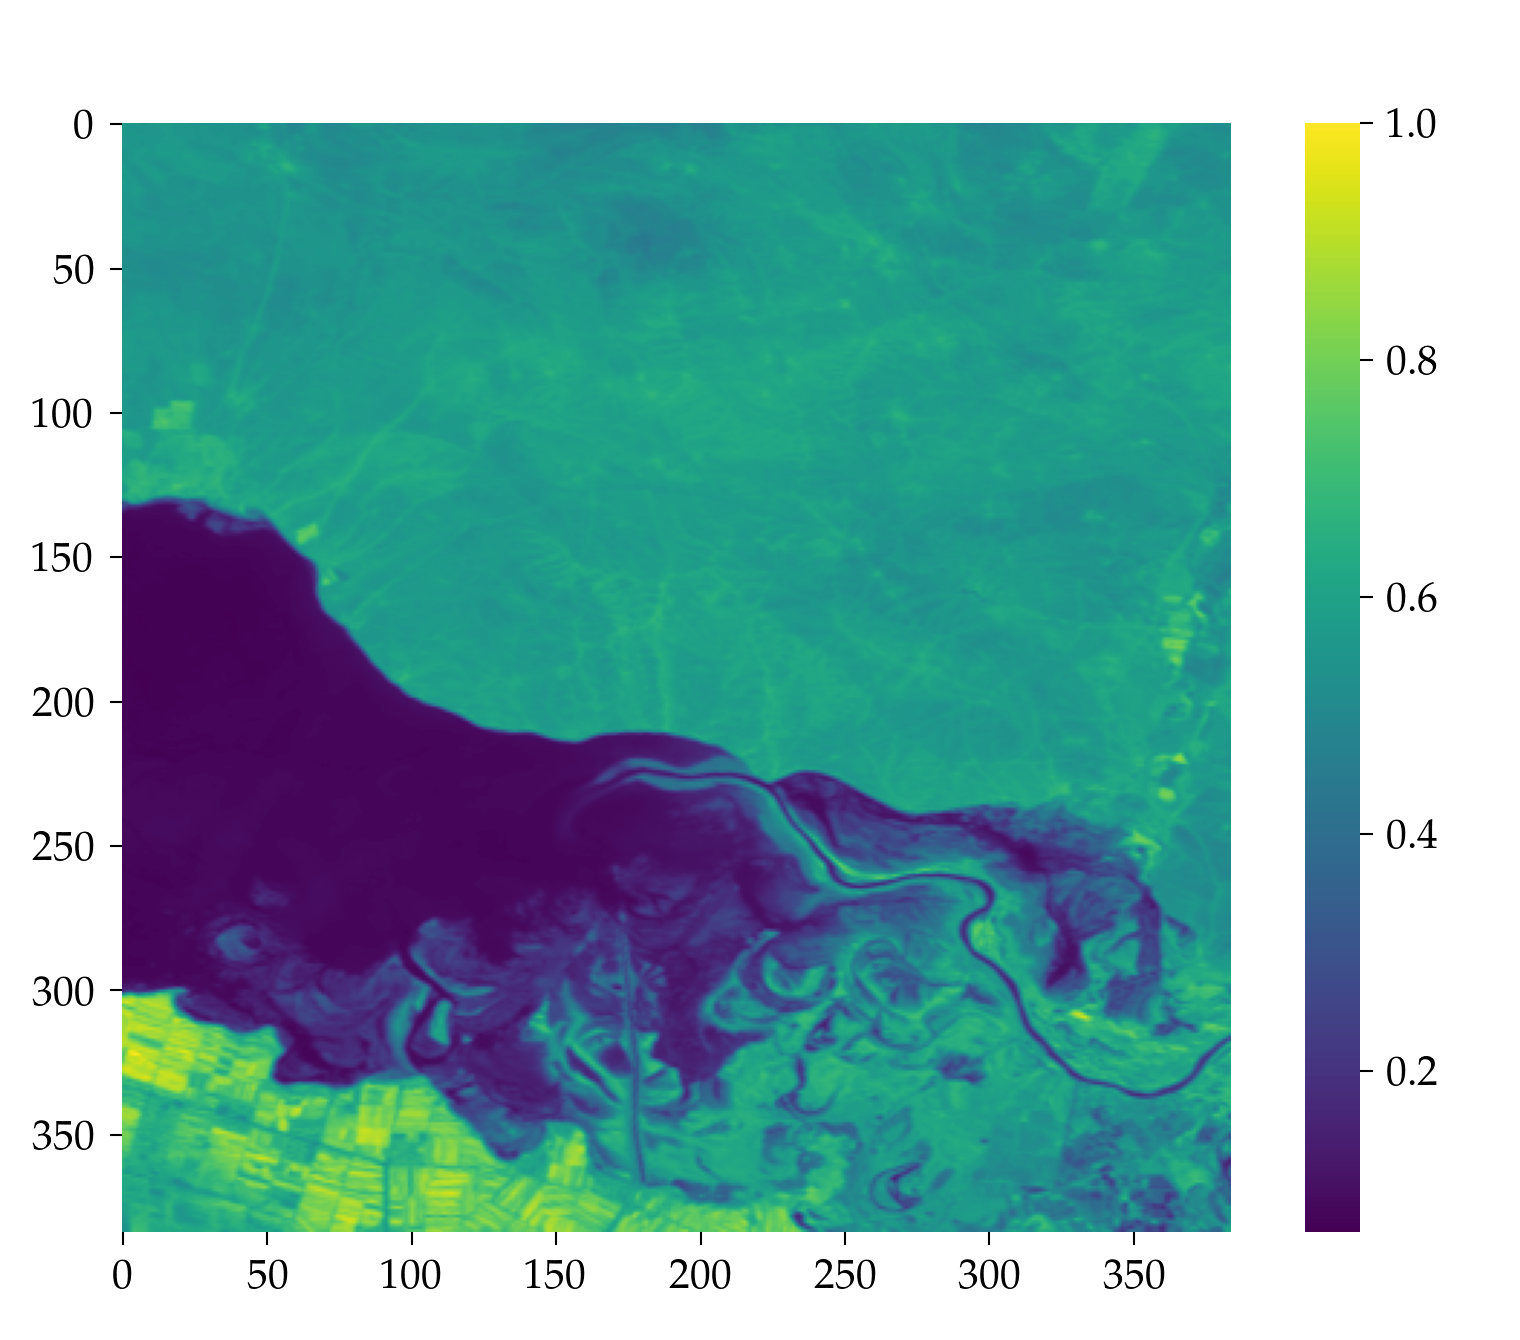
\includegraphics[width=0.75\textwidth]{viridis_demo_proba}
    \caption{An example of Proba-V satellite image with Viridis colormap applied}
    \label{fig:viridis}
\end{figure}

However, when comparing a number of side-by-side images it is important to apply the colormap consistently across all pictures.
Modern image processing libraries may try to stretch colormap to the range of the input image.
If images that are to be compared differ in maximal and minimal values, the way colormap is applied will be different.
It is important to ensure that images in the same scene display pixels with the same value in the same color.
For this reason, when several images are to be compared, they should be displayed with a common colormap.
At the same time, an outlier pixel in one of the images can result in the colormap not being well suited to display the rest of the pictures.
The solution to choosing a good colormap range is to use maximum and minimum values using pixel mean values and standard deviation:
\[ c_{max,min} = \bar{p} \pm 3 \cdot \sigma_p, \]
where $ c_{max,min} $ denotes maximum and minimum values of the color mappings, $ \bar{p} $ is the mean value of the pixels, and $ \sigma_p $ is the standard deviation of the pixel values.
This way, only pixels within the range of three standard deviations from the mean are taken into consideration when creating a common colormap for image comparison.